\documentclass[11pt]{article}
\usepackage[utf8]{inputenc}

\usepackage{graphicx}
\usepackage{fullpage}
\usepackage{framed}
\usepackage[spanish]{babel}

\begin{document}
\title{Manual de instalación de la librería \it Allegro 5 \rm para \it Microsoft Visual Studio 2015}
\author{Joaquin Olazabal, Dominic Schialer\\
			Programación I\\
			UPC}
\date{\today}
\maketitle
\vspace{50mm}
\tableofcontents
\pagebreak
\section{Introducción}
Allegro es una librería multiplataforma dirigida al desarrollo de videojuegos y programas multimedia. Maneja operaciones de bajo nivel como crear ventanas, leer el input del usuario, cargar datos, dibujar imágenes, reproducir sonidos, etc; generalmente abstrayendo la plataforma subyacente.  Sin embargo, Allegro \emph{no} es un motor de videojuego (game engine): eres libre de diseñar y estructurar tu programa a tu gusto.

\section{Instalación y configuración}
En Visual Studio seleccione \emph{File$>$New$>$Project}, nombre y cree un nuevo CLR Empty Project.
\subsection{Instalando Allegro}
Haga clic derecho en la solución y seleccione \emph{Manage NuGet Packages}(\emph{Fig.1}). A continuación, seleccione el tab \emph{Browse} e ingrese \emph{Allegro} en el buscador. El paquete principal de Allegro 5 se verá al inicio de la lista. Finalmente presione el botón \emph{Install} (\emph{Fig.2}). Una vez terminada la instalación deberá ver el mensaje de finalizado en la consola del output (\emph{Fig.3}).
\begin{center}
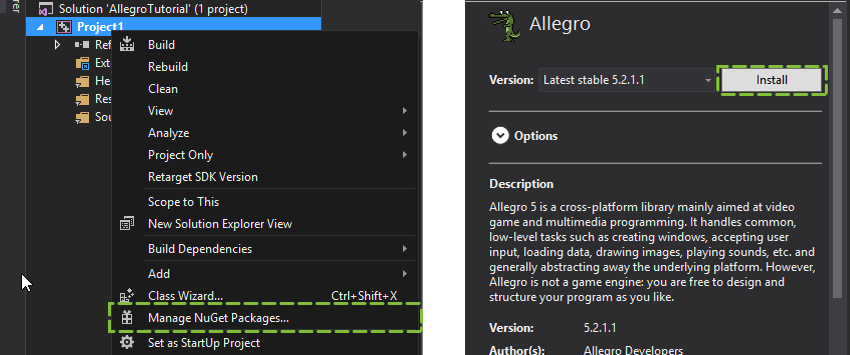
\includegraphics[scale=0.5]{SC23.png}

\emph{Figs.1 y 2}

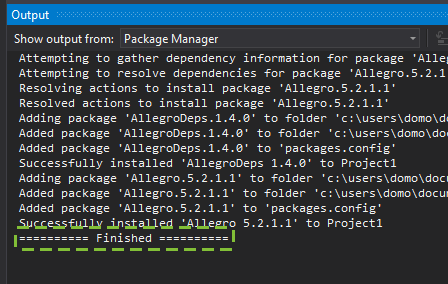
\includegraphics[scale=0.6]{SC4.png}
\ \emph{Fig.3}
\end{center}

\subsection{Configurando Allegro}
Para el primer ejemplo, proporcionado por \tt wiki.allegro.cc\rm , vamos a hacer uso de el addon de texto de Allegro llamado \emph{Font Addon}. Además configuraremos Allegro para que use debug y tiempo de ejecución dynámicos. La versión de debug le ayudará a verificar que esté usando Allegro de manera correcta, por eso se le recomienda seleccionarla durante el desarollo.

Haga clic derecho sobre la solución y seleccione \emph{Properties}. A continuación seleccione la entrada \emph{Allegro 5} y en \emph{Library Type} seleccione la opción \emph{Dynamic Debug - Dynamic Runtime} (\emph{Fig.4}).
En la entrada \emph{Add-ons} seleccione \emph{Yes} en \emph{Font Addon} (\emph{Fig.5}), para usar ese addon.\\
\begin{center}
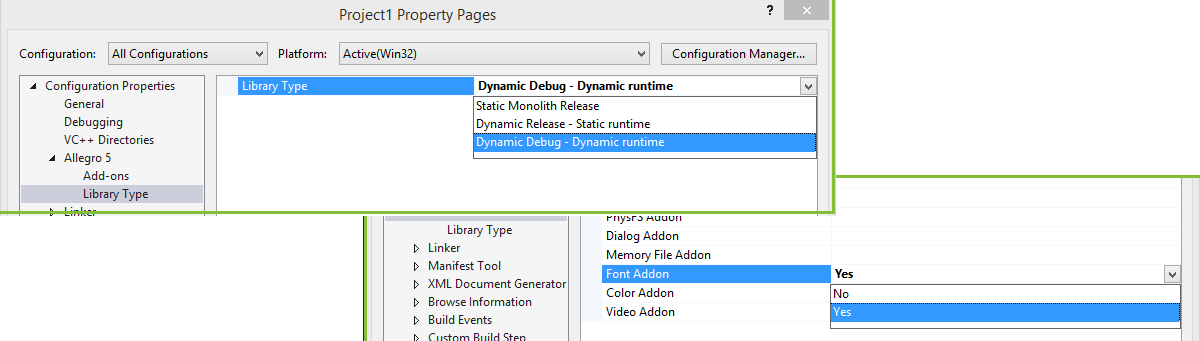
\includegraphics[scale=0.4]{SC67.png}
\ \emph{Figs.4 y 5}
\end{center}

\section{Ejemplos}
\subsection{Ejemplo 1: ¡Bienvenido a Allegro!}
Para verificar que todo funciona, cree un archivo source.cpp y copie el siguiente código.
\begin{verbatim}
#include <allegro5/allegro.h>
#include <allegro5/allegro_font.h>
 
int main()
{
     al_init();
     al_init_font_addon();
     ALLEGRO_DISPLAY* display = al_create_display(800, 600);
     ALLEGRO_FONT* font = al_create_builtin_font();
     al_clear_to_color(al_map_rgb(0, 0, 0));
     al_draw_text(font, al_map_rgb(255, 255, 255),
                         400, 300, ALLEGRO_ALIGN_CENTER, 
                         "Welcome to Allegro!");
     al_flip_display();
     al_rest(5.0);
     return 0;
}
\end{verbatim}
Al ejecutar, este código creará un a ventana e imprimirá la frase \emph{Welcome to Allegro!}, que depués de 5 segundos se cerrará.

\subsection{Ejemplo 2:  Visualización de una imagen}
En el siguiente ejemplo se mostrará como visualizar una imagen en Allegro. Para que pueda mostrar imagenes, se deberá usar el addon llamado \emph{Image Addon}, además de la configuración de \emph{Dynamic Debug - Dynamic Runtime} (véase sección 2.2). Todas las imágenes que sean utilizadas por el código deben de estar en la misma carpeta que el archivo source.cpp. De lo contrario Allegro no encontrará la imagen. El output del programa, según el código escrito, es el siguiente:
\begin{center}
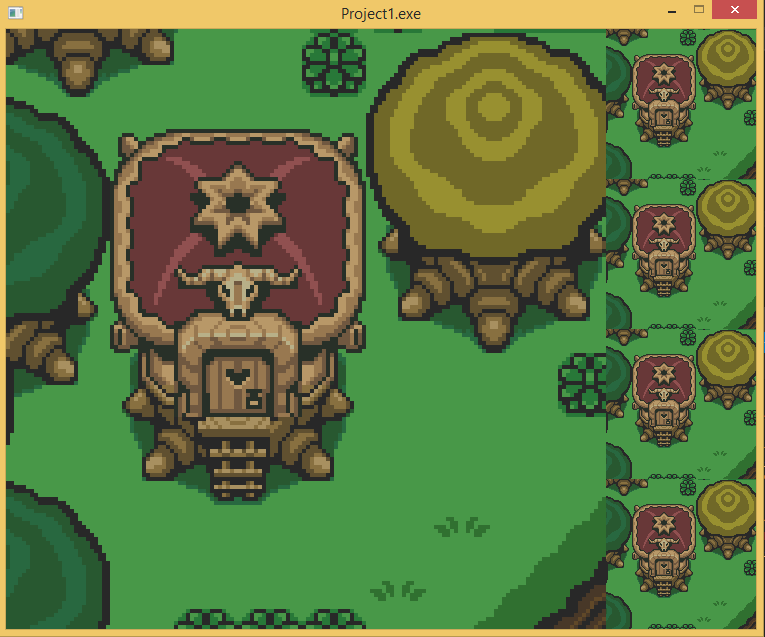
\includegraphics[scale=0.3]{SC12.png}
\end{center}
La imagen \tt test.png \rm con las dimesiones 150 x 150 px que se usará en este ejemplo se puede descargar de \tt http://i.imgur.com/5uoNsJs.png \rm .

\begin{verbatim}
#include <allegro5/allegro.h>
#include <allegro5/allegro_image.h>
\end{verbatim}
\fbox{ \parbox{\textwidth}{Las librerías necesarias son \emph{allegro.h}, la librería principal de Allegro, y \emph{allegro\_image.h}, la librería del addon de imágenes de Allegro. }}
\begin{verbatim}
int main() 
{
     al_init();
     al_init_image_addon();
\end{verbatim}
\fbox{\parbox{\textwidth}{Se inicializa Allegro y el addon de imágenes de Allegro.}}
\begin{verbatim}
     ALLEGRO_DISPLAY *display = NULL;
     ALLEGRO_BITMAP *fondo = al_load_bitmap("test.png");
     display = al_create_display(750, 600);
\end{verbatim}
\fbox{\parbox{\textwidth}{Se crean dos structs: \emph{ALLEGRO\_DISPLAY *display}, la ventana en la que el programa va a mostrar el output, y \emph{ALLEGRO\_BITMAP *fondo}, el bitmap que el programa usará.}}
\begin{verbatim}
     al_draw_scaled_bitmap(fondo, 0, 0, 150, 150, 0, 0, 600, 600, NULL);
     for (int i = 0; i<4;i++)
          al_draw_bitmap(fondo, 600, (150 * i), NULL);
\end{verbatim}
\fbox{\parbox{\textwidth}{Se dibujan los bitmaps en el buffer. \emph{al\_draw\_scaled\_bitmap()} tiene como argumentos el puntero del bitmap, la posición y tamaño del bitmap inicial, y la posición y tamaño del bitmap  modificado.}}
\begin{verbatim}
     al_flip_display();
\end{verbatim}
\fbox{\parbox{\textwidth}{Se 'vuelca' el buffer a la ventana.}}
\begin{verbatim}
     al_rest(10.0);
\end{verbatim}
\fbox{\parbox{\textwidth}{Se espera 10.0 segundos antes de ejecutar el resto del código.}}
\begin{verbatim}
     al_destroy_bitmap(fondo);
     al_destroy_display(display);
\end{verbatim}
\fbox{\parbox{\textwidth}{Finalmente se destruyen los structs, liberando así la memoria.}}
\begin{verbatim}
     return 0;
}
\end{verbatim}
\vfill
\begin{thebibliography}{9}
\bibitem{AllegroManual}
     Matthew Leverton, 
     Allegro 5.0 reference manual, 
     \verb!https://www.allegro.cc/manual/5/!, 
     \copyright 1999 - 2016,
     accedido: 25/09/2016
     
\bibitem{AllegroWiki}
     Allegro Wiki,
     \verb!https://wiki.allegro.cc!,
     accedido: 25/09/2016
\end{thebibliography}

\end{document}